\subsection{Анализ затрат на изготовление продукта}

Затраты на выполнение проекта включают оплату труда исполнителей, расходы на приобретение оборудования, затраты на организацию рабочих мест, а также накладные расходы, связанные с обеспечением процесса разработки. Данный анализ позволяет оценить экономическую целесообразность создания программного продукта и определить основные статьи расходов, оказывающие наибольшее влияние на итоговую стоимость проекта.

Проектные затраты определяются по формуле \eqref{eq:K}.

\begin{equation}\label{eq:K}
K = C_{\text{ЗАРП}} + C_{\text{ОБ}} + C_{\text{ОРГ}} + C_{\text{НАКЛ}},
\end{equation}
где $C_{\text{ЗАРП}}$ -- заработная плата исполнителей; \\ $C_{\text{ОБ}}$ -- затраты на обеспечение необходимым оборудованием; \\ $C_{\text{ОРГ}}$ -- затраты на организацию рабочих мест; \\ $C_{\text{НАКЛ}}$ -- накладные расходы.

\subsubsection{Затраты на заработную плату}

Затраты на заработную плату исполнителей определяются по формуле \eqref{eq:Czarp}.

\begin{equation}\label{eq:Czarp}
C_{\text{ЗАРП}} = C_{\text{ОСН}} + C_{\text{ДОП}} + C_{\text{ОТЧ}},
\end{equation}
где $C_{\text{ОСН}}$ -- основная заработная плата; \\ $C_{\text{ДОП}}$ -- дополнительная заработная плата; \\ $C_{\text{ОТЧ}}$ -- отчисления с заработной платы.

Расчет основной заработной платы при дневной оплате труда проводится на основе данных по окладам и графику занятости исполнителей. Её расчет выполняется согласно формуле  \eqref{eq:Cosn}.

\begin{equation}\label{eq:Cosn}
C_{\text{ОСН}} = T_{\text{ЗАН}} \cdot O_{\text{ДН}},
\end{equation}
где $T_{\text{ЗАН}}$ -- число дней, отработанных исполнителем проекта; \\ $O_{\text{ДН}}$ -- дневной оклад исполнителя.

При восьмичасовом рабочем дне дневной оклад определяется по формуле \eqref{eq:Odn}.

\nopagebreak
\begin{equation}\label{eq:Odn}
O_{\text{ДН}} = \frac{8 \cdot O_{\text{МЕС}}}{F_{\text{М}}},
\end{equation}
где $O_{\text{МЕС}}$ -- месячный оклад; \\ $F_{\text{М}}$ -- месячный фонд рабочего времени.

Месячный оклад вычисляется с учётом налога на доходы физических лиц по формуле \eqref{eq:Omes}.

\begin{equation}\label{eq:Omes}
O_{\text{МЕС}} = O \cdot \left(1 + \frac{\text{Н}_{\text{НДФЛ}}}{100}\right),
\end{equation}
где $O$ -- чистый оклад; \\ $\text{Н}_{\text{НДФЛ}}$ -- налог на доходы физических лиц, равный 13\% для большинства налогоплательщиков.

Месячный фонд рабочего времени принят на основании производственного календаря на 2026 год. При 40-часовой рабочей неделе годовая норма рабочего времени составляет 1972 часа, следовательно,

$$
F_{\text{М}} = \frac{1972}{12} = 164.3 \ \text{час./мес.}
$$

После составления графика работ определены уровни заработной платы исполнителей в соответствии с формулой \eqref{eq:Cosn}. Для расчётов использованы данные HeadHunter. Средний чистый месячный оклад инженера принят равным 125000 рублей, а аналитика данных -- 104400 рублей. Тогда месячный и дневной оклад для инженера составляют 141250 рублей и 6876.3 рубля, а для аналитика -- 117972 рубля и 5743.1 рубля соответственно.

Подробные результаты представлены в таблице~\ref{tab:salary_calc}.

\begin{table}[h!]
    \centering
    \caption{Расчёт затрат на заработную плату исполнителей}
    \label{tab:salary_calc}
    \begin{tabular}{|p{3.2cm}|c|c|c|c|c|}
        \hline
        Исполнитель & $T_{\text{ЗАН}}$, дн. & $O$, руб. & $O_{\text{МЕС}}$, руб. & $O_{\text{ДН}}$, руб./дн. & $C_{\text{ОСН}}$, руб. \\
        \hline
        Инженер & 97.5 & 125000 & 141250 & 6876.3 & 670439.25 \\
        \hline
        Аналитик данных & 31.0 & 104400 & 117972 & 5743.1 & 178036.1 \\
        \hline
    \end{tabular}
\end{table}

Дополнительно произведено уточнение затрат на заработную плату на основе расчётов в КСП-системе. Объём затрат на основную заработную плату для инженера составил 670439{,}25 рубля за 780 часов работы, а для аналитика -- 178036{,}1 рубля за 248 часов работы. Тогда суммарная основная заработная плата определяется по формуле \eqref{eq:Cosn_total}.

\begin{equation}\label{eq:Cosn_total}
C_{\text{ОСН}} = 670439{,}25 + 178036{,}1 = 848475{,}35 \ \text{руб.}
\end{equation}

Дополнительная заработная плата учитывает выплаты за время, не связанное с производственной деятельностью, но предусмотренное законодательством,  в том числе: оплата очередных отпусков, компенсация за недоиспользованный отпуск, и др.. Она определяется по формуле \eqref{eq:Cdop}.

\begin{equation}\label{eq:Cdop}
C_{\text{ДОП}} = 0.2 \cdot C_{\text{ОСН}}.
\end{equation}

Тогда дополнительная заработная плата $C_{\text{ДОП}}$ равна:
$$
C_{\text{ДОП}} = 0.2 \cdot 848475{,}35 = 169695{,}07 \ \text{руб.}
$$

Отчисления с заработной платы состоят в настоящее время в уплате единого социального налога. Согласно налоговому кодексу РФ применяются ставки налога для отчисления в пенсионный фонд РФ, фонд социального страхования, фонды обязательного медицинского страхования и рассчитываются по формуле \eqref{eq:Cotch}.

\begin{equation}\label{eq:Cotch}
C_{\text{ОТЧ}} = \text{Н}_{\text{СОЦ}} \cdot (C_{\text{ОСН}} + C_{\text{ДОП}}),
\end{equation}
где $\text{Н}_{\text{СОЦ}}$ -- страховые взносы, составляющие 30\% от выплат и включающие:

\begin{itemize}
    \item пенсионное страхование -- 22\%;
    \item социальное страхование -- 2{,}9\%;
    \item медицинское страхование -- 5{,}1\%.
\end{itemize}

Тогда

$$
C_{\text{ОТЧ}} = 0.3 \cdot (848475{,}35 + 169695{,}07) = 305451{,}13 \ \text{руб.}
$$

Общие затраты на заработную плату исполнителям составляют:
$$
C_{\text{ЗАРП}} = 848475{,}35 + 169695{,}07 + 305451{,}13 = 1323621{,}55 \ \text{руб.}
$$

\subsubsection{Затраты на материалы и оборудование}

Затраты на материалы и оборудование включают расходы на рабочие станции, вычислительный сервер и доступ к сети Интернет. Поскольку в ходе разработки используется преимущественно программное обеспечение с открытым исходным кодом, лицензионные отчисления в состав материальных затрат не включаются.

Общие затраты на материалы и оборудование представлены в таблице~\ref{tab:materials_costs}.

\begin{table}[h!]
    \centering
    \caption{Затраты на материалы и оборудование}
    \label{tab:materials_costs}
    \begin{tabular}{|p{5.8cm}|c|c|}
        \hline
        Наименование & Количество & Стоимость, руб. \\
        \hline
        Ноутбук HUAWEI MateBook D 16 (i5-12450H, 16GB, 512GB SSD) для инженера-программиста & 1 & 52\,824 \\
        \hline
        Ноутбук ASUS VivoBook 15 X1502ZA (i5-1235U, 16GB, 512GB SSD) для аналитика & 1 & 51\,940 \\
        \hline
        GPU-сервер с видеокартой NVIDIA RTX 4090 24 ГБ & 1 & 887\,217 \\
        \hline
        Доступ к сети Интернет на период разработки & 1 & 9\,000 \\
        \hline
        Итого & -- & 1\,000\,981 \\
        \hline
    \end{tabular}
\end{table}

Для выполнения работ по анализу audit-логов и разработке модели обнаружения аномалий требуются два рабочих места: для инженера и для аналитика. В качестве рабочих станций выбраны ноутбуки HUAWEI MateBook D 16 и ASUS VivoBook 15, оснащённые процессорами Intel Core i5, 16 ГБ оперативной памяти и SSD-накопителями объёмом 512 ГБ. Данные характеристики достаточны для разработки, тестирования и предобработки данных.

Для обучения и проверки модели обнаружения аномалий необходим вычислительный сервер с графическим ускорителем NVIDIA RTX 4090 24 ГБ. Для проекта принят GPU-сервер стоимостью 887\,217 руб., обеспечивающий достаточную производительность для ресурсоёмких операций машинного обучения.

Расходы на доступ к сети Интернет приняты укрупнённо из расчёта 1\,500 руб. в месяц на период шести месяцев разработки, что составляет 9\,000 руб.

Таким образом, общая величина затрат на материалы и оборудование определяется по формуле \eqref{eq:Cmat}.

\begin{equation}
C_{\text{МАТ}} = 52\,824 + 51\,940 + 887\,217 + 9\,000 = 1\,000\,981 \ \text{руб.}
\label{eq:Cmat}
\end{equation}

Затраты на амортизацию оборудования определяются по формуле:

\begin{equation}
C_{\text{АМОРТ}} = \sum_{i=1}^{n} \left( C_{\text{об}i} \cdot \frac{\Delta t_i}{D_i} \right),
\end{equation}
где $C_{\text{об}i}$ — стоимость $i$-го оборудования; \\ $\Delta t_i$ — время использования оборудования в днях; \\ $D_i$ — срок службы оборудования в днях.

Срок выполнения проекта составляет 6 месяцев (180 дней). Срок службы ноутбуков и сервера принят равным 5 годам (1825 дней).

Тогда затраты на амортизацию составляют:

$$
C_{\text{АМОРТ}} =
\frac{52\,824 \cdot 180}{1825} +
\frac{51\,940 \cdot 180}{1825} +
\frac{887\,217 \cdot 180}{1825}
= 97\,834{,}4 \ \text{руб.}
$$

\subsubsection{Затраты на организацию рабочих мест и накладные расходы}

Общепроизводственные расходы включают затраты на обслуживание, организацию работ и управление проектом. При организации рабочих мест с ПЭВМ необходимо соблюдать санитарные нормы по площади и объёму помещения, а также по взаимному размещению рабочих мест.

На основе анализа предложений аренды коммерческой недвижимости были рассмотрены несколько вариантов помещений. Для проекта выбран вариант, обеспечивающий размещение двух рабочих мест и принтера при приемлемом уровне затрат.

\begin{longtable}{|p{3.2cm}|c|c|c|}
    \caption{Анализ вариантов аренды помещения для размещения рабочих мест} 
    \label{tab:rental_analysis} \\ \hline
    Адрес помещения & Площадь, кв.\,м & Аренда в месяц, руб.  \\ \hline
    \endfirsthead

    \caption*{Продолжение таблицы \ref{tab:rental_analysis}} \\ \hline
    Адрес помещения & Площадь, кв.\,м & Аренда в месяц, руб. \\ \hline
    \endhead

    \hline
    \endfoot

    \hline
    \endlastfoot

    Бизнес-парк «Румянцево (Корпус Е)» & 25 & 35\,417  \\ \hline
    Бизнес-парк «Румянцево (Корпус Е)» & 83 & 117\,583 \\ \hline
    Москва, Нижегородская 32А & 20 & 14\,287  \\ \hline
    Москва, Дмитровское шоссе 98с1 & 23 & 140\,304 \\ \hline
\end{longtable}

По результатам анализа выбран вариант помещения площадью 20~кв.\,м и стоимостью 14\,287 руб. в месяц. При сроке выполнения проекта 6 месяцев затраты на организацию рабочих мест составляют 85\,722 руб.

\begin{equation}
C_{\text{ОРГ}} = 14\,287 \cdot 6 = 85\,722 \ \text{руб.}
\end{equation}

Накладные расходы, связанные с выполнением проекта, определяются на основе затрат на основную заработную плату исполнителей. В соответствии с принятой практикой они составляют 60\% от основной заработной платы.

Тогда накладные расходы определяются по формуле:

$$
C_{\text{НАКЛ}} = 0.6 \cdot C_{\text{ОСН}}
$$

Подставляя рассчитанное значение основной заработной платы, получаем:

$$
C_{\text{НАКЛ}} = 0.6 \cdot 848475{,}35 = 509085{,}21 \ \text{руб.}
$$


\subsubsection{Анализ расходов}

По данным таблицы \ref{tab:all_costs}, суммарные затраты на реализацию проекта составляют 3\,017\,244{,}16 руб. Наибольшую долю в структуре расходов занимает заработная плата исполнителей — 1\,323\,621{,}55 руб., что составляет около 43,9\% от общей суммы затрат. Это объясняется высокой трудоёмкостью разработки программного средства, включающей анализ предметной области, проектирование архитектуры, реализацию модулей, тестирование и подготовку документации.

Второй по величине статьёй расходов является закупка оборудования. На неё приходится 1\,000\,981 руб., или около 33,2\% от общей стоимости проекта. Значительная доля данной статьи связана с необходимостью приобретения рабочих станций для исполнителей, а также вычислительного сервера, используемого для обучения и проверки модели обнаружения аномалий. Таким образом, материально-техническое обеспечение оказывает существенное влияние на общую стоимость проекта.

\begin{table}[h!]
  \centering
  \caption{Суммарные затраты по статьям расходов}
  \label{tab:all_costs}
  \begin{tabular}{|c|l|r|}
    \hline
    № & Статья расходов & Затраты, руб. \\
    \hline
    1 & Заработная плата & 1\,323\,621{,}55 \\ \hline
    2 & Закупка оборудования & 1\,000\,981 \\ \hline
    3 & Амортизация оборудования & 97\,834{,}4 \\ \hline
    4 & Аренда помещения & 85\,722 \\ \hline
    5 & Накладные расходы & 509\,085{,}21 \\ \hline
    \multicolumn{2}{|r|}{\textbf{Итого}} & \textbf{3\,017\,244{,}16} \\
    \hline
  \end{tabular}
\end{table}

На рисунке \ref{fig:cost_chart} представлена диаграмма, отражающая структуру затрат на изготовление продукта.

\begin{figure}[h!]
  \centering
  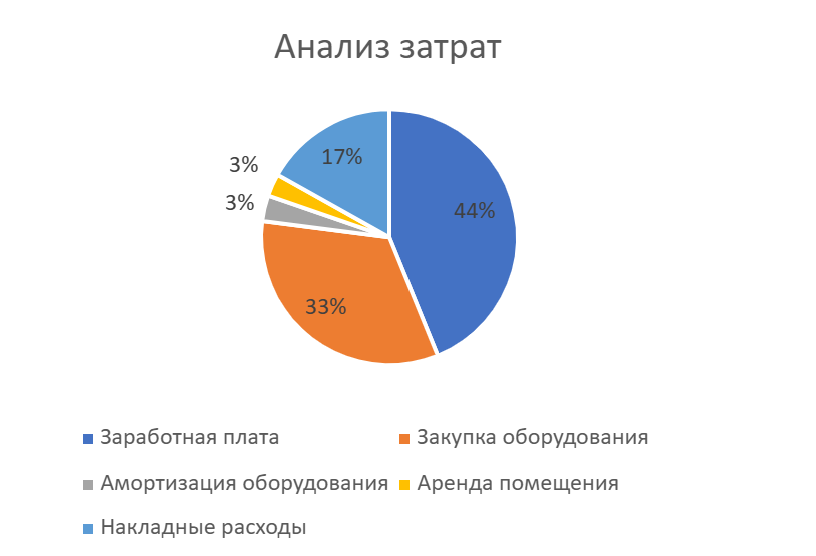
\includegraphics[scale=1]{inc/images/cost_chart}
  \caption{Диаграмма структуры затрат на изготовление продукта}
  \label{fig:cost_chart}
\end{figure}
